\chapter{Testing \& Results}
This chapter details the testing that was carried out to assess the performance of different parts of the system, such as the human detection and direction, as well as the powered wheelchair and Hololens system as a whole. We outline the test setups used to evaluate the performance of the systems, as well as the results of the tests and what they imply about the implemented system.

\section{Human Detection and Distance}
This section is concerned with testing the Human Detection \& Direction system and the Hologram GameObject placement. To ensure the system will be able to detect real people moving around in the surroundings, it is necessary to test the system detecting people at different distances and the directions they are facing. We also want to test the accuracy of the spatial mapping system in terms of correcting the real world positions of the GameObjects representing the detected people. We utilize the Microsoft Hololens and the HDD system for this test.

\subsection{Test System Description} \label{sec:hddSys}
As explained in the Implementation chapter of this report, the front facing camera uses ROS topics to stream video frames to a partner computer the HDD system is implemented on. The HDD processes the frames and detects people and determines whether they are facing the PWU or not. The bounding box of the detections and directions are sent back to the Unity application. Initially, the application converts the pixel co-ordinates of the detections to corresponding world co-ordinates. We then use the spatial mapping and ray casting capabilities of the Hololens to correct the world position distances of the holograms representing the detected people.

\subsection{Test Setup} \label{sec:testSetup}
We setup a testing ground in the ICRS Lab on the 5th floor of the EEE building. We marked out points at 1 meter intervals which indicate where the target people should stand. We asked the person wearing the Hololens to sit down in a chair to emulate the position and height a PWU would be at when sitting in the wheelchair. Figure \ref{fig:hddTestSetup} shows the experimental setup in the lab. For this step, all subjects were stationary, except when the target person moves between the markings.

\begin{figure}[ht]
	\centering
	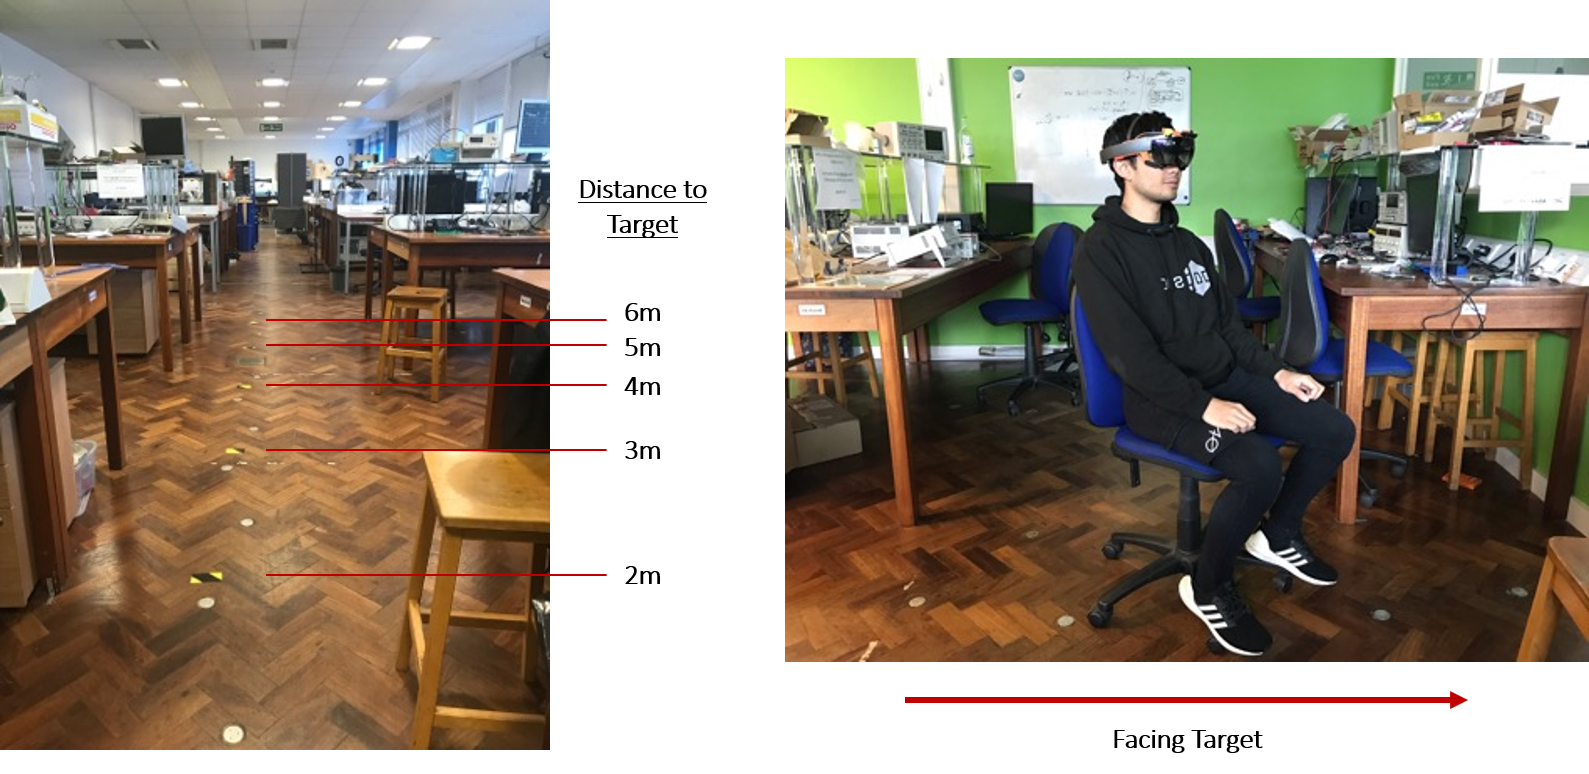
\includegraphics[width=1.0\linewidth]{img/chapter6_test/hddTestSetup.png}
	\caption{The experimental setup used to test the HDD and Hololens spatial mapping accuracy. We asked the people acting as targets to stand at 1 meter intervals while a person sitting down wearing the Hololens looked at them using the front facing camera.}
	\label{fig:hddTestSetup}
\end{figure}
 
We modified the Hololens Unity application to display holograms showing the distance between the Hololens and the target person in meters. We asked the person wearing the Hololens to call out the value the hologram displayed as the target person stood at different markings. To verify the readings, we recorded the Hololens display using the Windows Device Portal and watched them over after the test. Recording the hololens view also allowed us to see how the distance reading change as the target person moves.
 
\subsection{Test Procedure}
We asked three different people to sit in the chair and wear the Hololens. Before commencing the test, we allowed the people to learn how to wear the Hololens properly, ensuring the Hololens was correctly placed on the bridge of the users nose. We also allowed them to do several test detections to familiarise them with how the distance holograms would be rendered. This was done so that each participant would be able to detect the target person and call out the distance displayed by the hologram.

\paragraph{} The selected people all had different amounts of experience with the Hololens. One user was a complete novice, putting the Hololens on for the first time to participate in the test. One was an intermediate, having worn the Hololens a few times during the development of this project and the last person was more experienced with the Hololens and how the HDD system would detect the target people.

\paragraph{} We asked the target person to face forward at each marker, before turning their back and facing away from the Hololens user. This was done to check if there were any differences between the placement accuracy of the GameObjects for different orientations of the person.

\subsection{Results}
We show the results of the experiment in Figure \ref{fig:hddResults}, which compares the accuracy of hologram placement after spatial mapping and ray casting with the true world position of the detected person. Each test subject was given several seconds to adjust their head positions to ensure a detection was achieved. Despite this, none of the three test subjects were able to get holographic distances for a target at $6$m or further. This may indicate that the system was unable to detect a person at that distance, but what is more likely  is that the spatial mapping of the Hololens was unable to detect a surface that far away to render the distance hologram on. By looking at the debug log messages in Visual Studio 2017, we verified that there were indeed detections at $6$m, but they returned inaccurate values distance values.

\begin{figure}[ht]
	\centering
	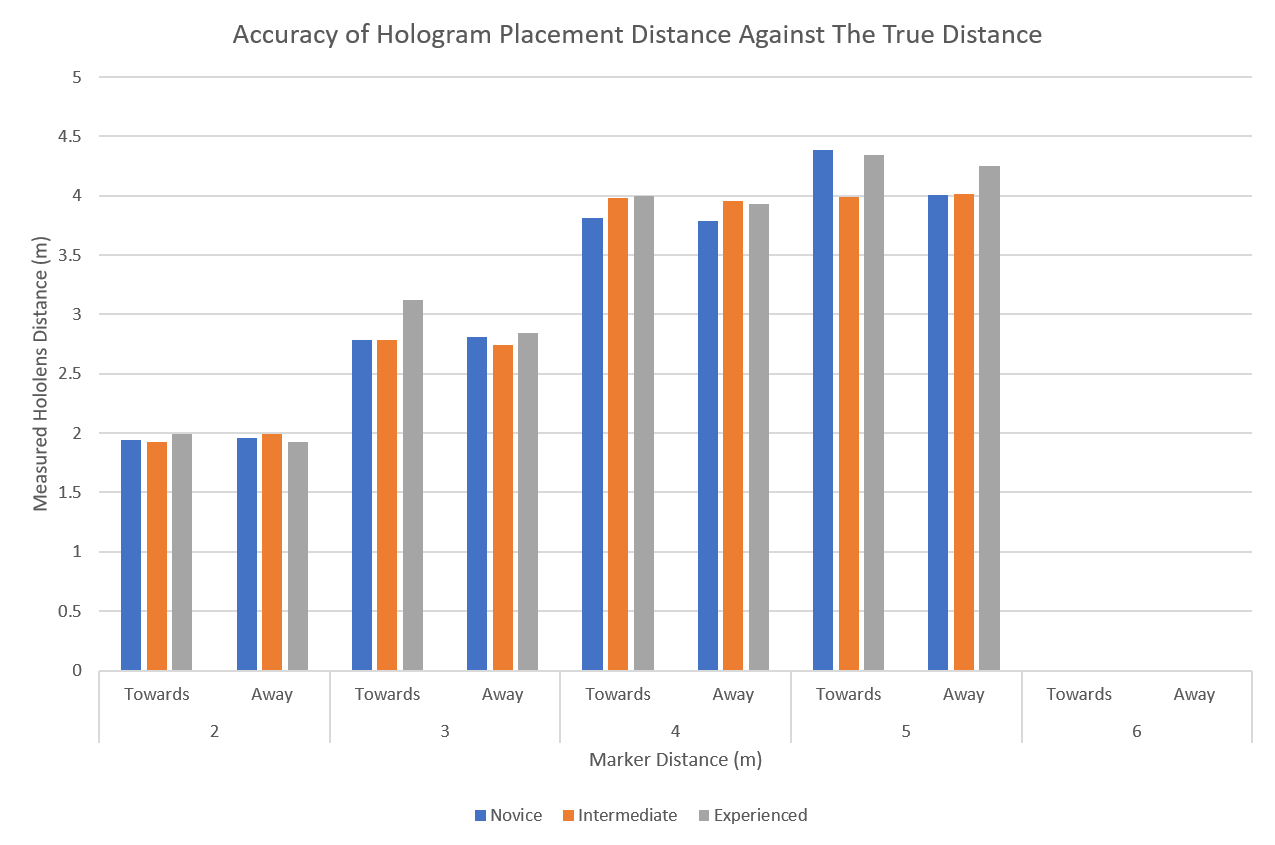
\includegraphics[width=1.0\linewidth]{img/chapter6_test/hddtestresults.png}
	\caption{The graph shows that there is no significant difference between the orientation of the target. We note the decrease in accuracy past $4$m, and the lack of holograms at $6$m.}
	\label{fig:hddResults}
\end{figure}

The data shows that there is no significant difference in hologram placement distance for target persons facing towards or away from the Hololens. However, we note that the hologram placement accuracy decreases the further away the target person is from the Hololens. This is further shown from the Hololens view recordings in Figure \ref{fig:marek}, whereby we can see that the placement of the hologram is not on the target person, but a surface just behind the target.

\begin{figure}[ht]
	\begin{subfigure}[b]{.32\textwidth}
		\centering
		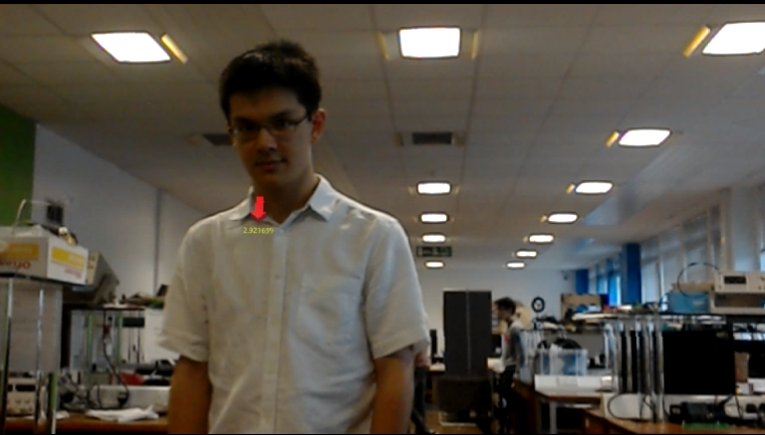
\includegraphics[width=1.0\linewidth]{img/chapter6_test/marek.png}
		\caption{Subject at 2m}
	\end{subfigure}%
	\hspace{\fill} 
	\begin{subfigure}[b]{.32\textwidth}
		\centering
		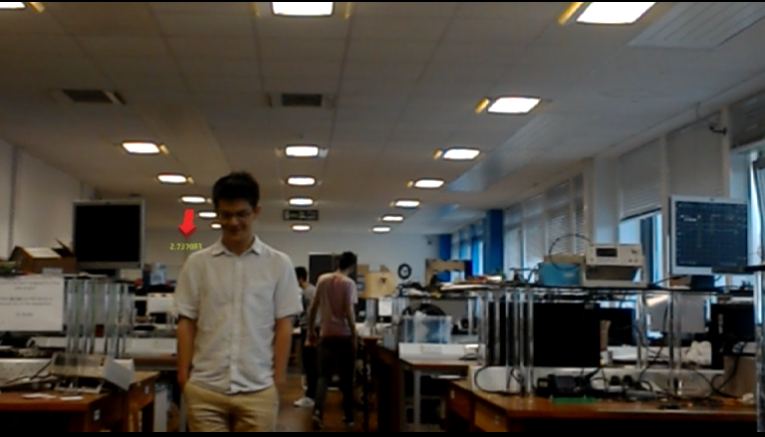
\includegraphics[width=1.0\linewidth]{img/chapter6_test/marek1.png}
		\caption{Subject at 3m}
	\end{subfigure}
	\hspace{\fill} 
	\begin{subfigure}[b]{.32\textwidth}
		\centering
		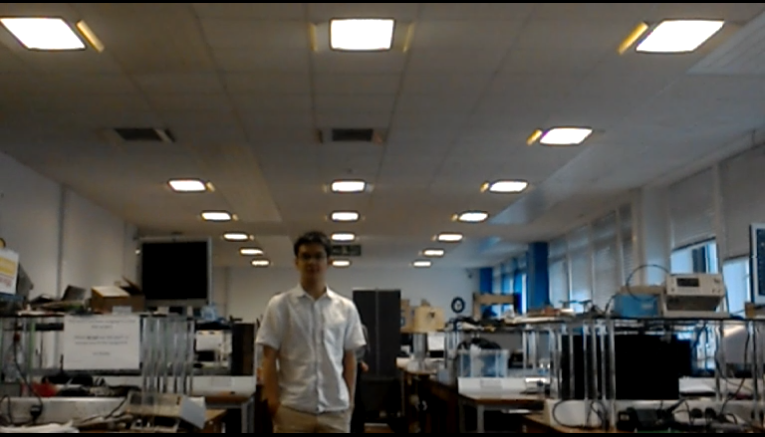
\includegraphics[width=1.0\linewidth]{img/chapter6_test/marek2.png}
		\caption{Subject at 6m}
	\end{subfigure}
	\vspace{-1\baselineskip}
	\begin{center}
		\caption{Target person at different distances viewed through the front-camera of the Hololens. We note that the accuracy of the hologram placement decreases as the target is further away.}
		\label{fig:marek}
	\end{center}
	\vspace{-2\baselineskip}
\end{figure}

\paragraph{} After the test, we asked the test subjects on qualitative feedback on how easy it it is to view a hologram. As expected, the novice Hololens user had difficulty seeing holograms due to the limited FOV of the device. The novice stated that the holograms were being rendered too high up, as they could only see the bottom of the hologram, as the rest of it was slightly out of view unless they tilted their head upwards. The intermediate user had a similar experience, but only had difficulty in seeing the holograms when the target person was closer than 2 meters.

\subsection{Discussion} \label{sec:distanceDiscussion}
From our results, we note that the test subjects were unable to see a hologram when the target person was more than 5m away, which indicates that there is a limitation with the spatial mapping of the Hololens. We suspect that this is due to a surface mesh not being rendered for the detected person, since the spatial mapping class was unable to discern between the person and the background at that distance. Secondly, we bring up the issue of hologram placement accuracy compared to the real world position of the target person. This issue is visualized by the graph in Figure \ref{fig:hddResults}, which shows a drop in accuracy for distances beyond 4 meters. Furthermore, Figure \ref{fig:marek}.b shows the hologram being rendered on a surface behind the target person.

\paragraph{} We believe that these issues are caused by ray casting through an incorrect world co-ordinate. Firstly, The frames captured by the front facing camera have to be compressed and streamed to a partner PC. The frames are then processed by the HDD system before being streamed back across the network. The culmination of the time spent being processed and streamed means that there is a slight delay between the detection of the person and their current position as interpreted by the Hololens. As such, when the Hololens un-projects the image co-ordinate of the detection to obtain a world co-ordinate, the placement of the initial GameObject is slightly incorrect. The system uses the ray casting function to pass a ray through the current position and expects the spatial mapping to detect a surface representing the detected person to position the hologram on. However, due to the slight delay, the ray continues to travel until it hits the background mesh instead of the person. This would explain why holograms are correctly placed on detections which are nearer, since the person is larger in the frame, and as such, has more surface mesh area for the ray cast to hit.

\section{Gazebo Simulation} \label{sec:gazeboSimTest}
Before testing the system using ARTA in the real world, we used the robot simulation tool Gazebo to test how the reactive control system would manipulate the ARTA control signals in response to person detections at different distances. The purpose of this simulation is to test the communication between ARTA and the Hololens, and how the reactive control system manipulates the velocity of the wheelchair as it approaches a detected person. We also want to test if the system can decide if the detections are to the side of the wheelchair or in front, and react appropriately. 

\subsection{Test System Description}
For this test, we use the same system as the one described in Section \ref{sec:hddSys}, with the addition of the Gazebo simulation of the ARTA powered wheelchair. We communicate the ARTA control signals to the Hololens, which checks the trajectory of the wheelchair and determines if a collision with a detected person is imminent. If the reactive control system decides a detected person is a collision risk, it reduces the velocity of the wheelchair in order to avoid a collision.

\subsection{Test Setup}

\subsubsection{Gazebo Simulation}
We use the Gazebo Simulation software to load a world built using the height map for the hallway outside the Personal Robotics Lab on the 10th floor. We then load the Unified Robot Description Format (URDF) model of ARTA into the world and run the ROS nodes controlling the powered wheelchair. We control the simulated wheelchair using the keyboard on the computer instead of a joystick.

\begin{figure}[ht]
	\begin{subfigure}[b]{.48\textwidth}
		\centering
		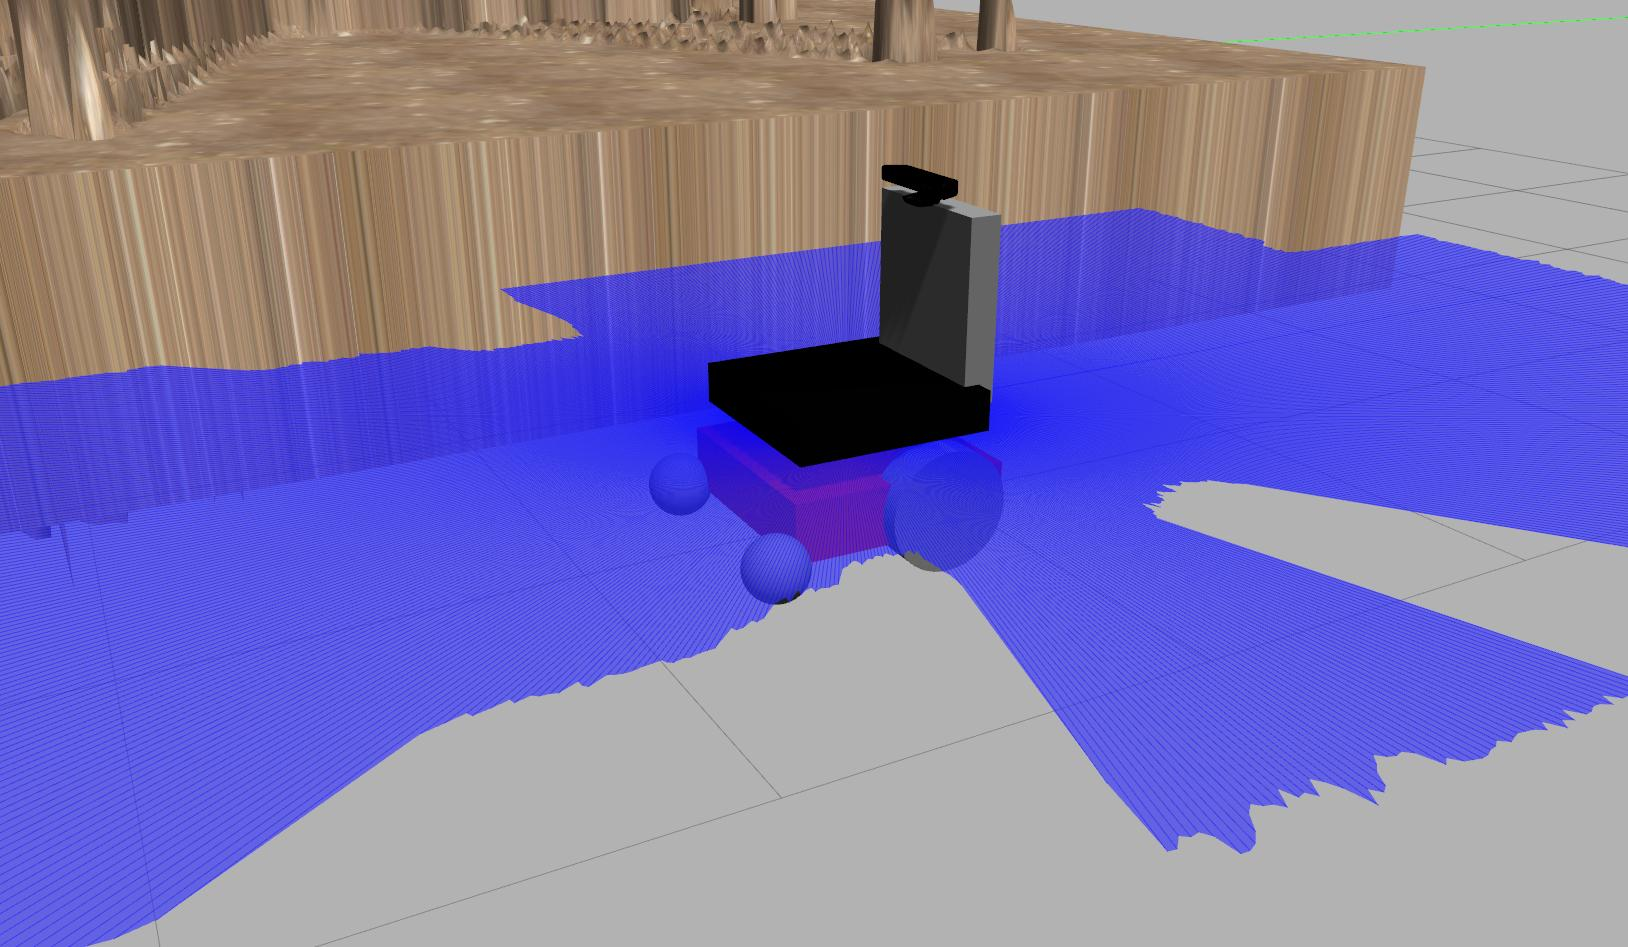
\includegraphics[width=1.0\linewidth]{img/chapter6_test/artamodel.jpg}
		\caption{URDF model of ARTA with joints that model the kinematics of the wheelchair.}
	\end{subfigure}%
	\hspace{\fill} 
	\begin{subfigure}[b]{.48\textwidth}
		\centering
		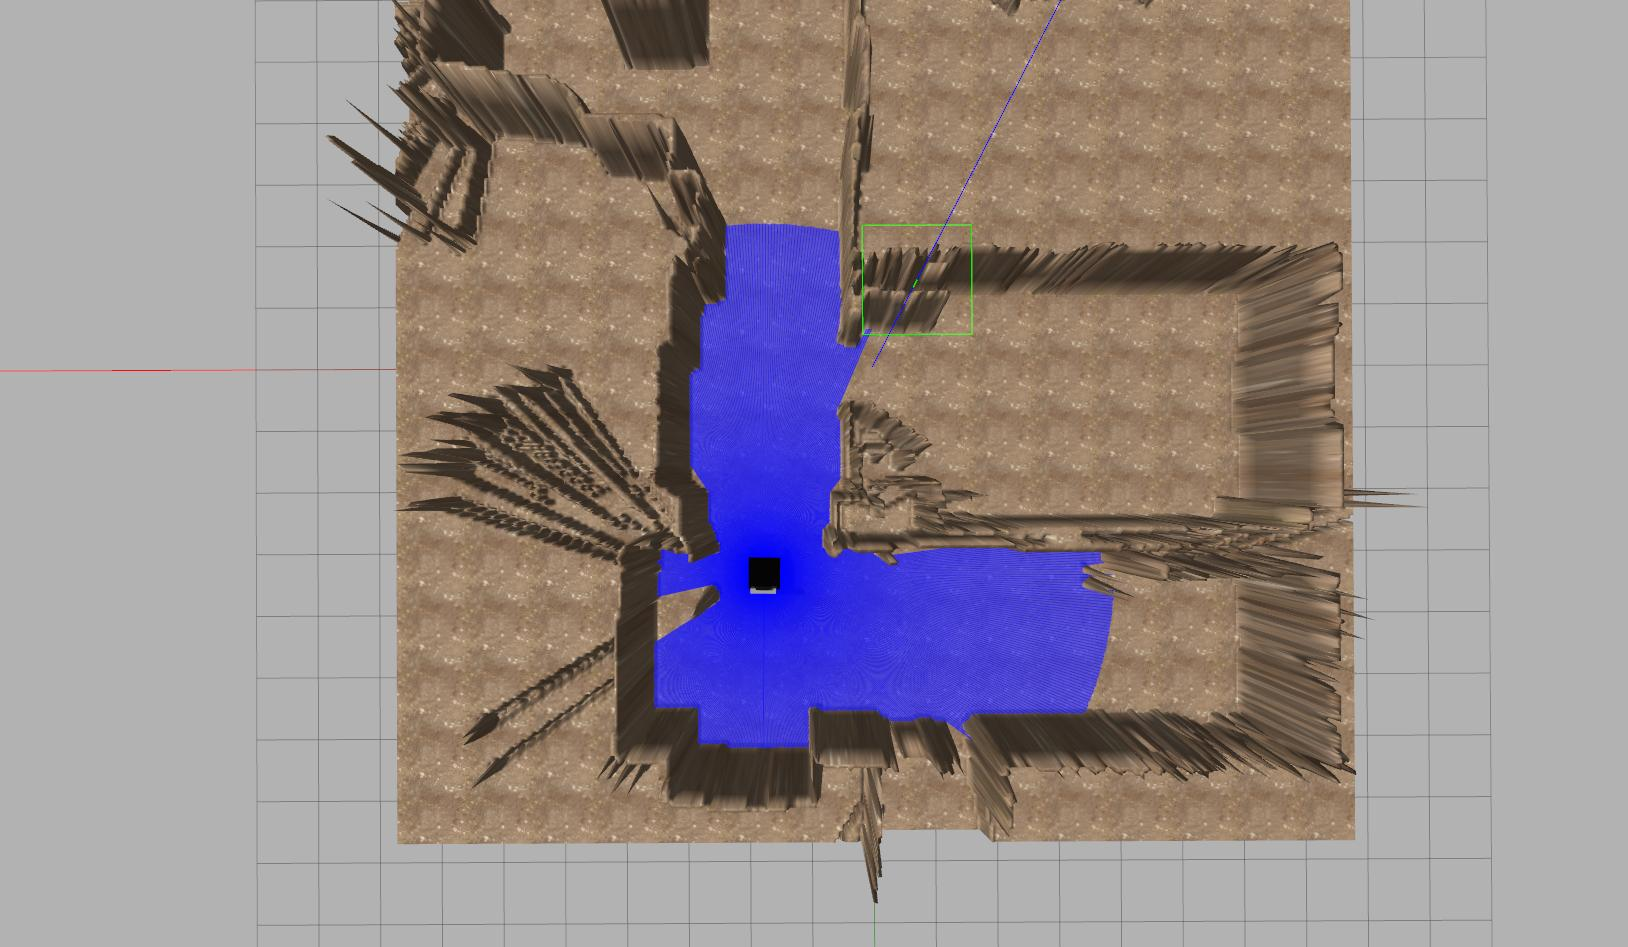
\includegraphics[width=1.0\linewidth]{img/chapter6_test/heightmap.jpg}
		\caption{An aerial view of the Lab Hallway on the 10th floor.}
	\end{subfigure}
	\vspace{-1\baselineskip}
	\begin{center}
		\caption{The Gazebo Simulation of the lab hallway outside the PRL. The blue mesh represents the range of the simulated laser scanner.}
		\label{fig:greenredrender}
	\end{center}
	\vspace{-1\baselineskip}
\end{figure}

\begin{figure}[ht!]
	\begin{subfigure}[b]{.48\textwidth}
		\centering
		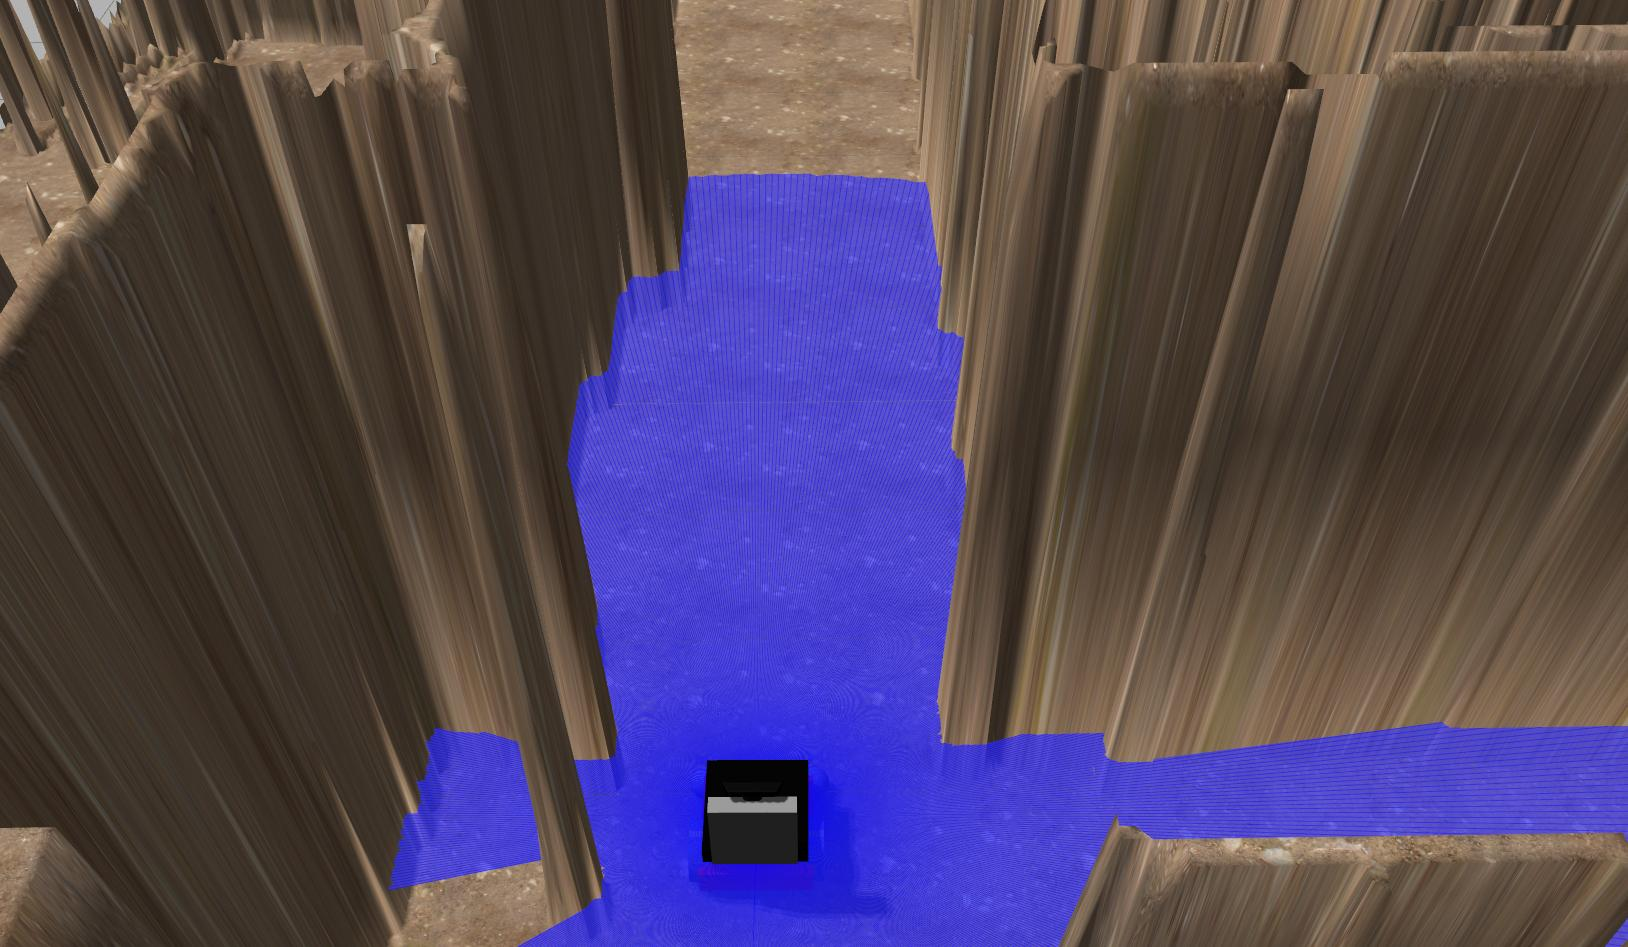
\includegraphics[width=1.0\linewidth]{img/chapter6_test/gazeboBack.jpg}
		\caption{Gazebo Simulation of hallway from behind the model.}
	\end{subfigure}%
	\hspace{\fill} 
	\begin{subfigure}[b]{.48\textwidth}
		\centering
		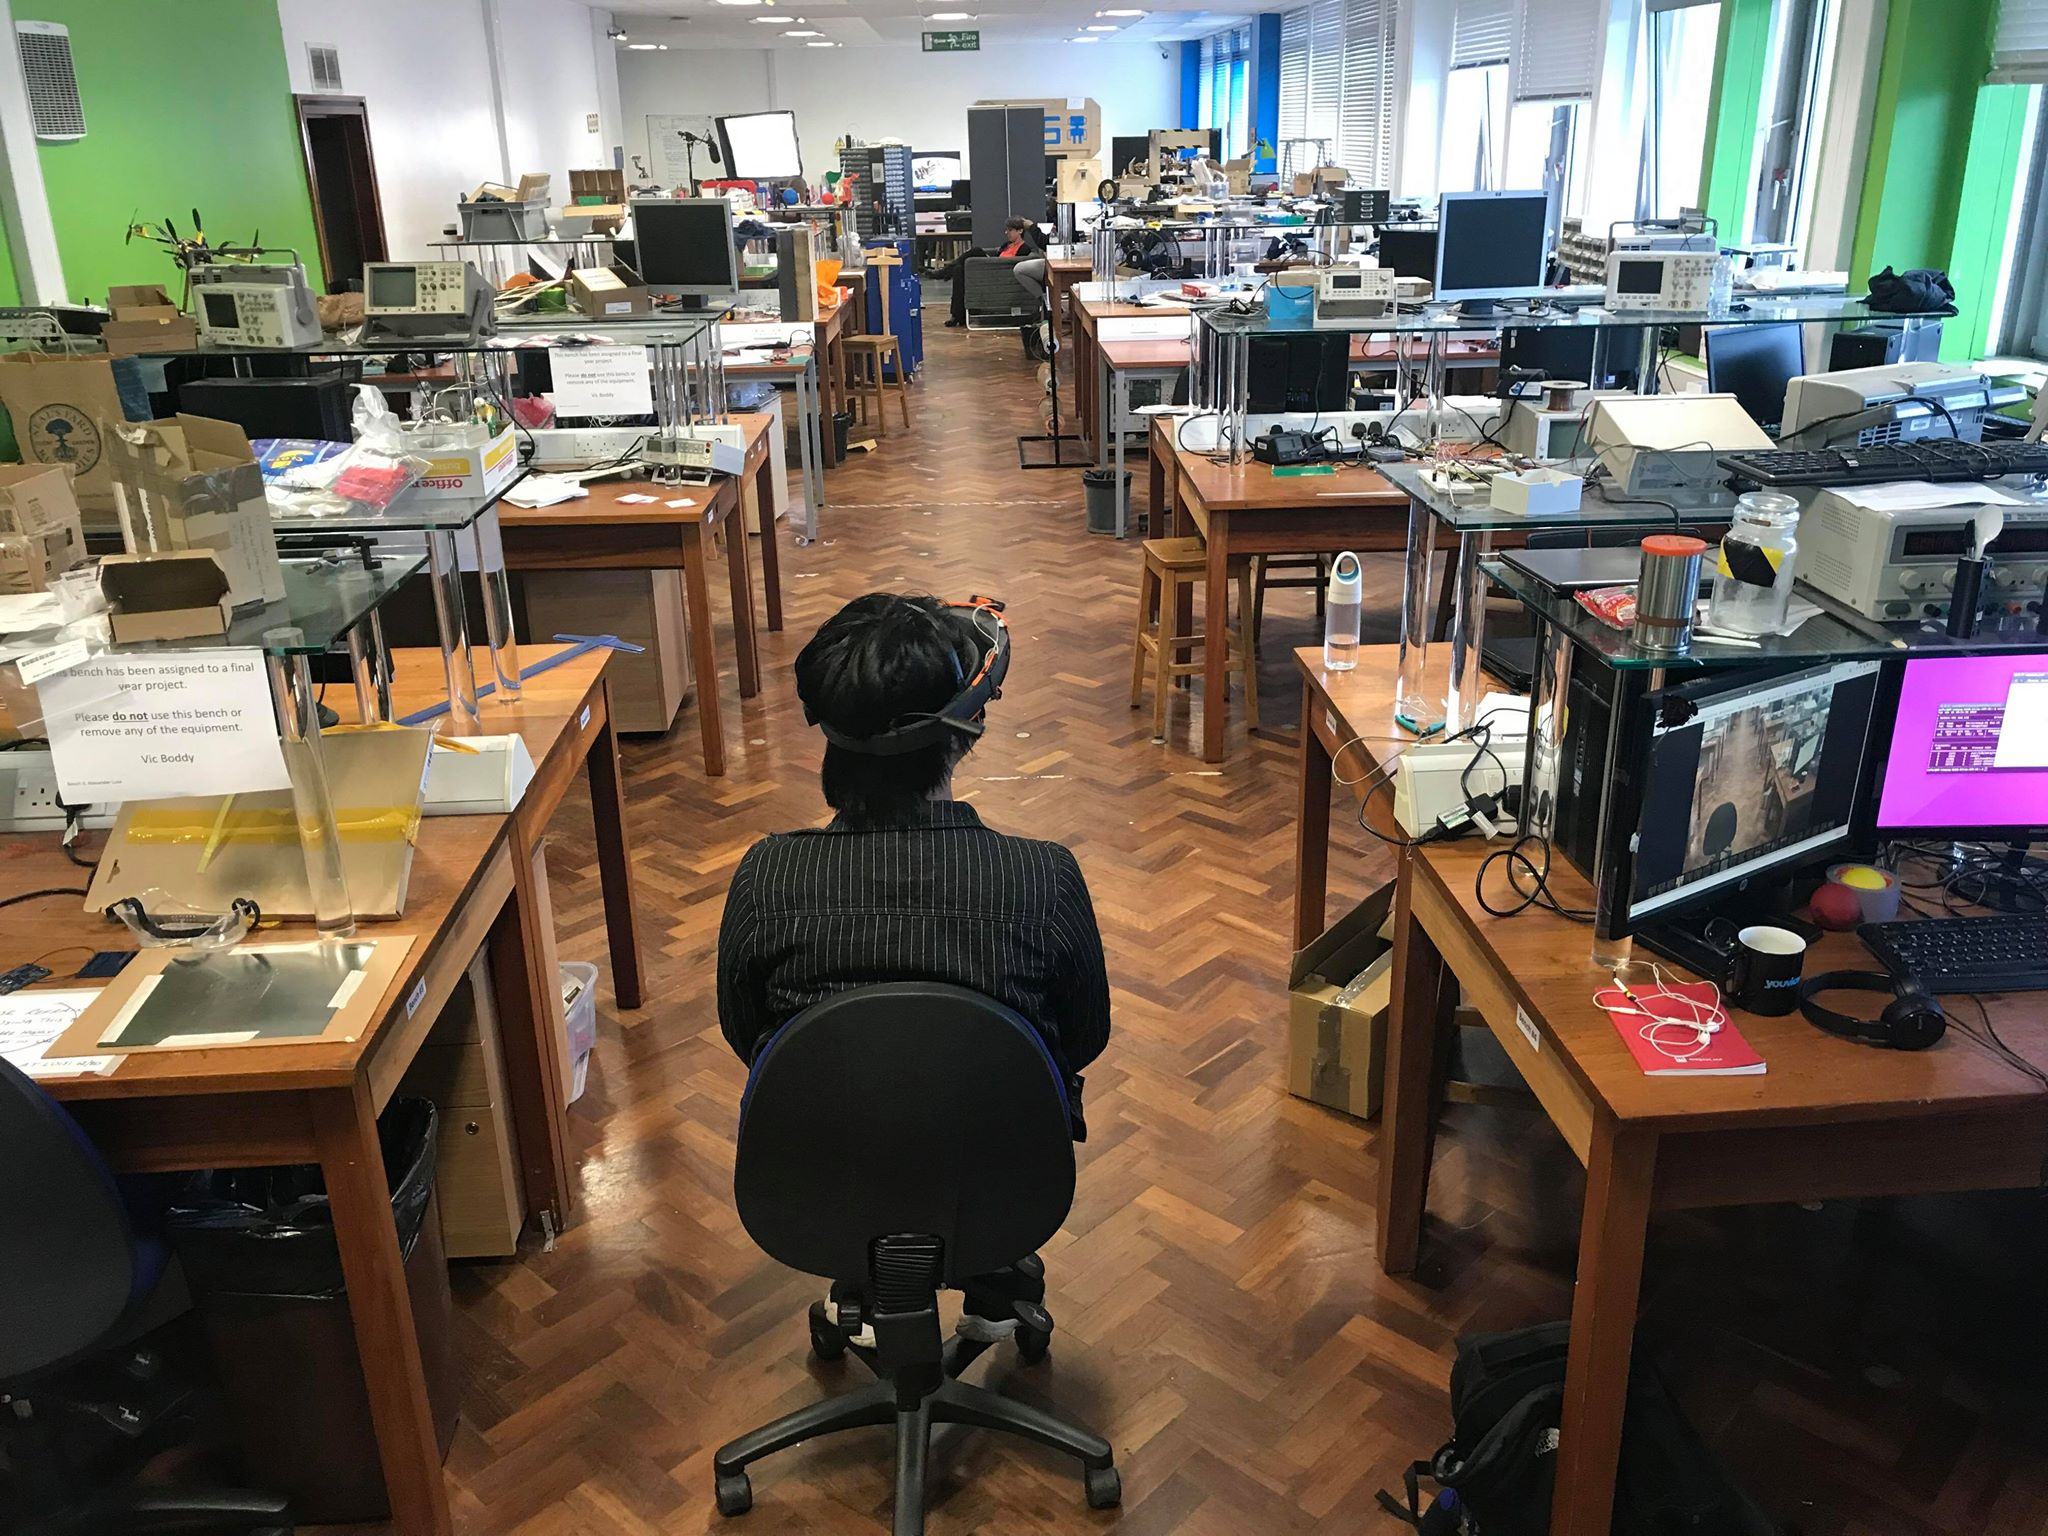
\includegraphics[width=1.0\linewidth,height=41.5mm]{img/chapter6_test/realBack.jpg}
		\caption{Corresponding real world lab setup from behind.}
	\end{subfigure}

	\begin{subfigure}[b]{.48\textwidth}
		\centering
		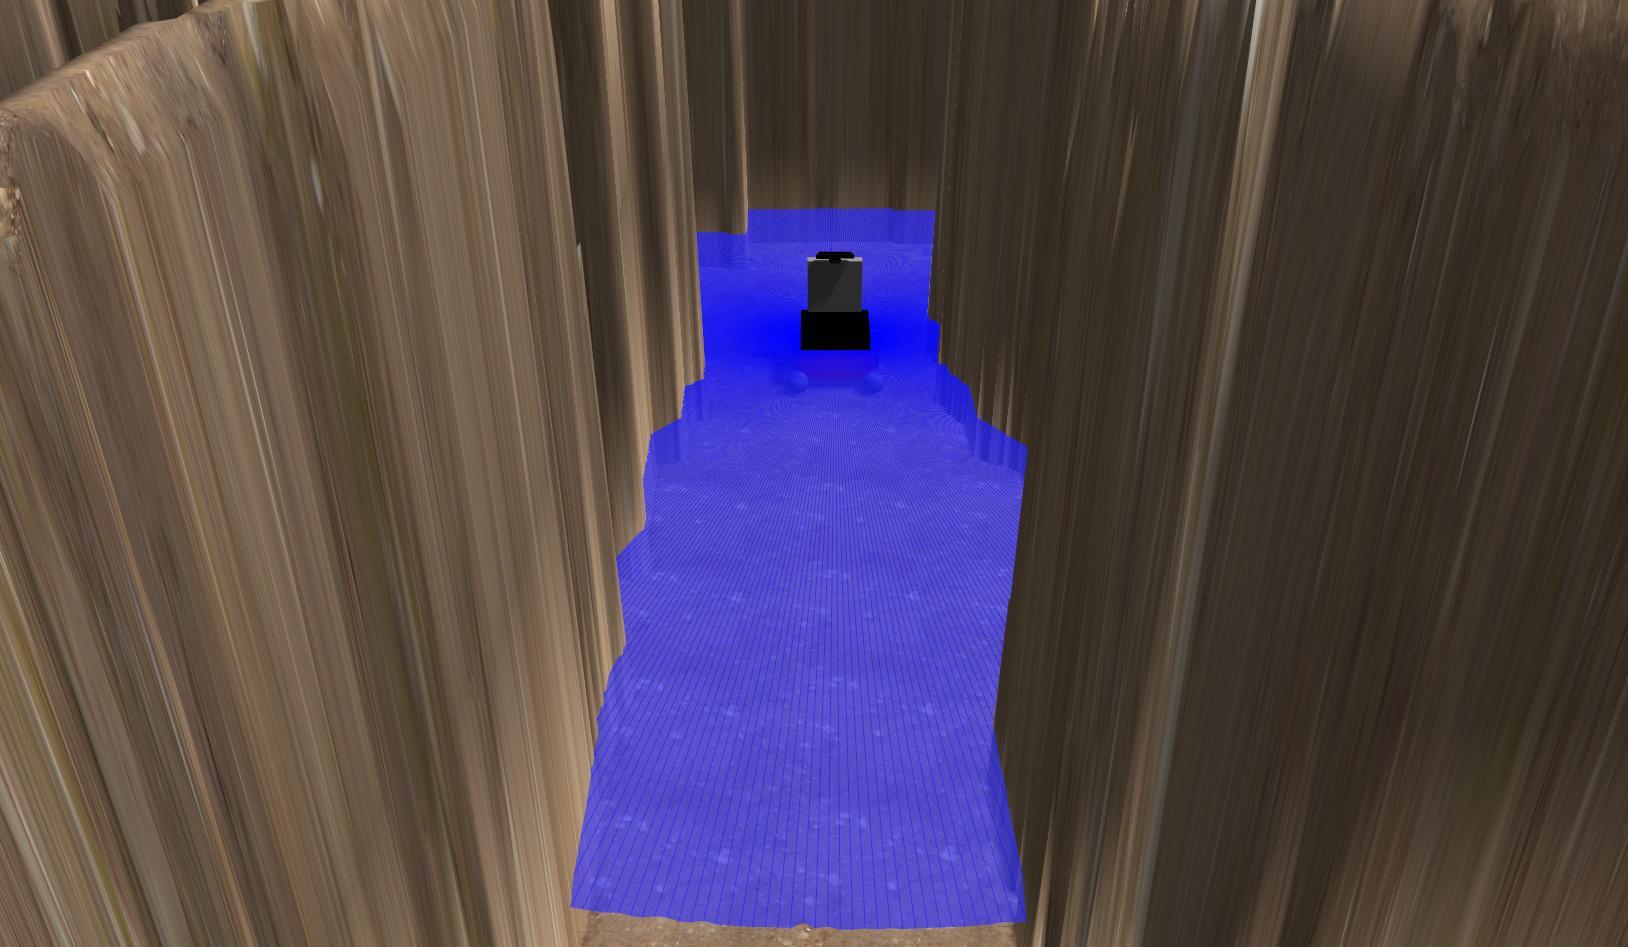
\includegraphics[width=1.0\linewidth]{img/chapter6_test/gazeboFront.jpg}
		\caption{Gazebo Simulation of hallway from in front of the model.}
	\end{subfigure}%
	\hspace{\fill} 
	\begin{subfigure}[b]{.48\textwidth}
		\centering
		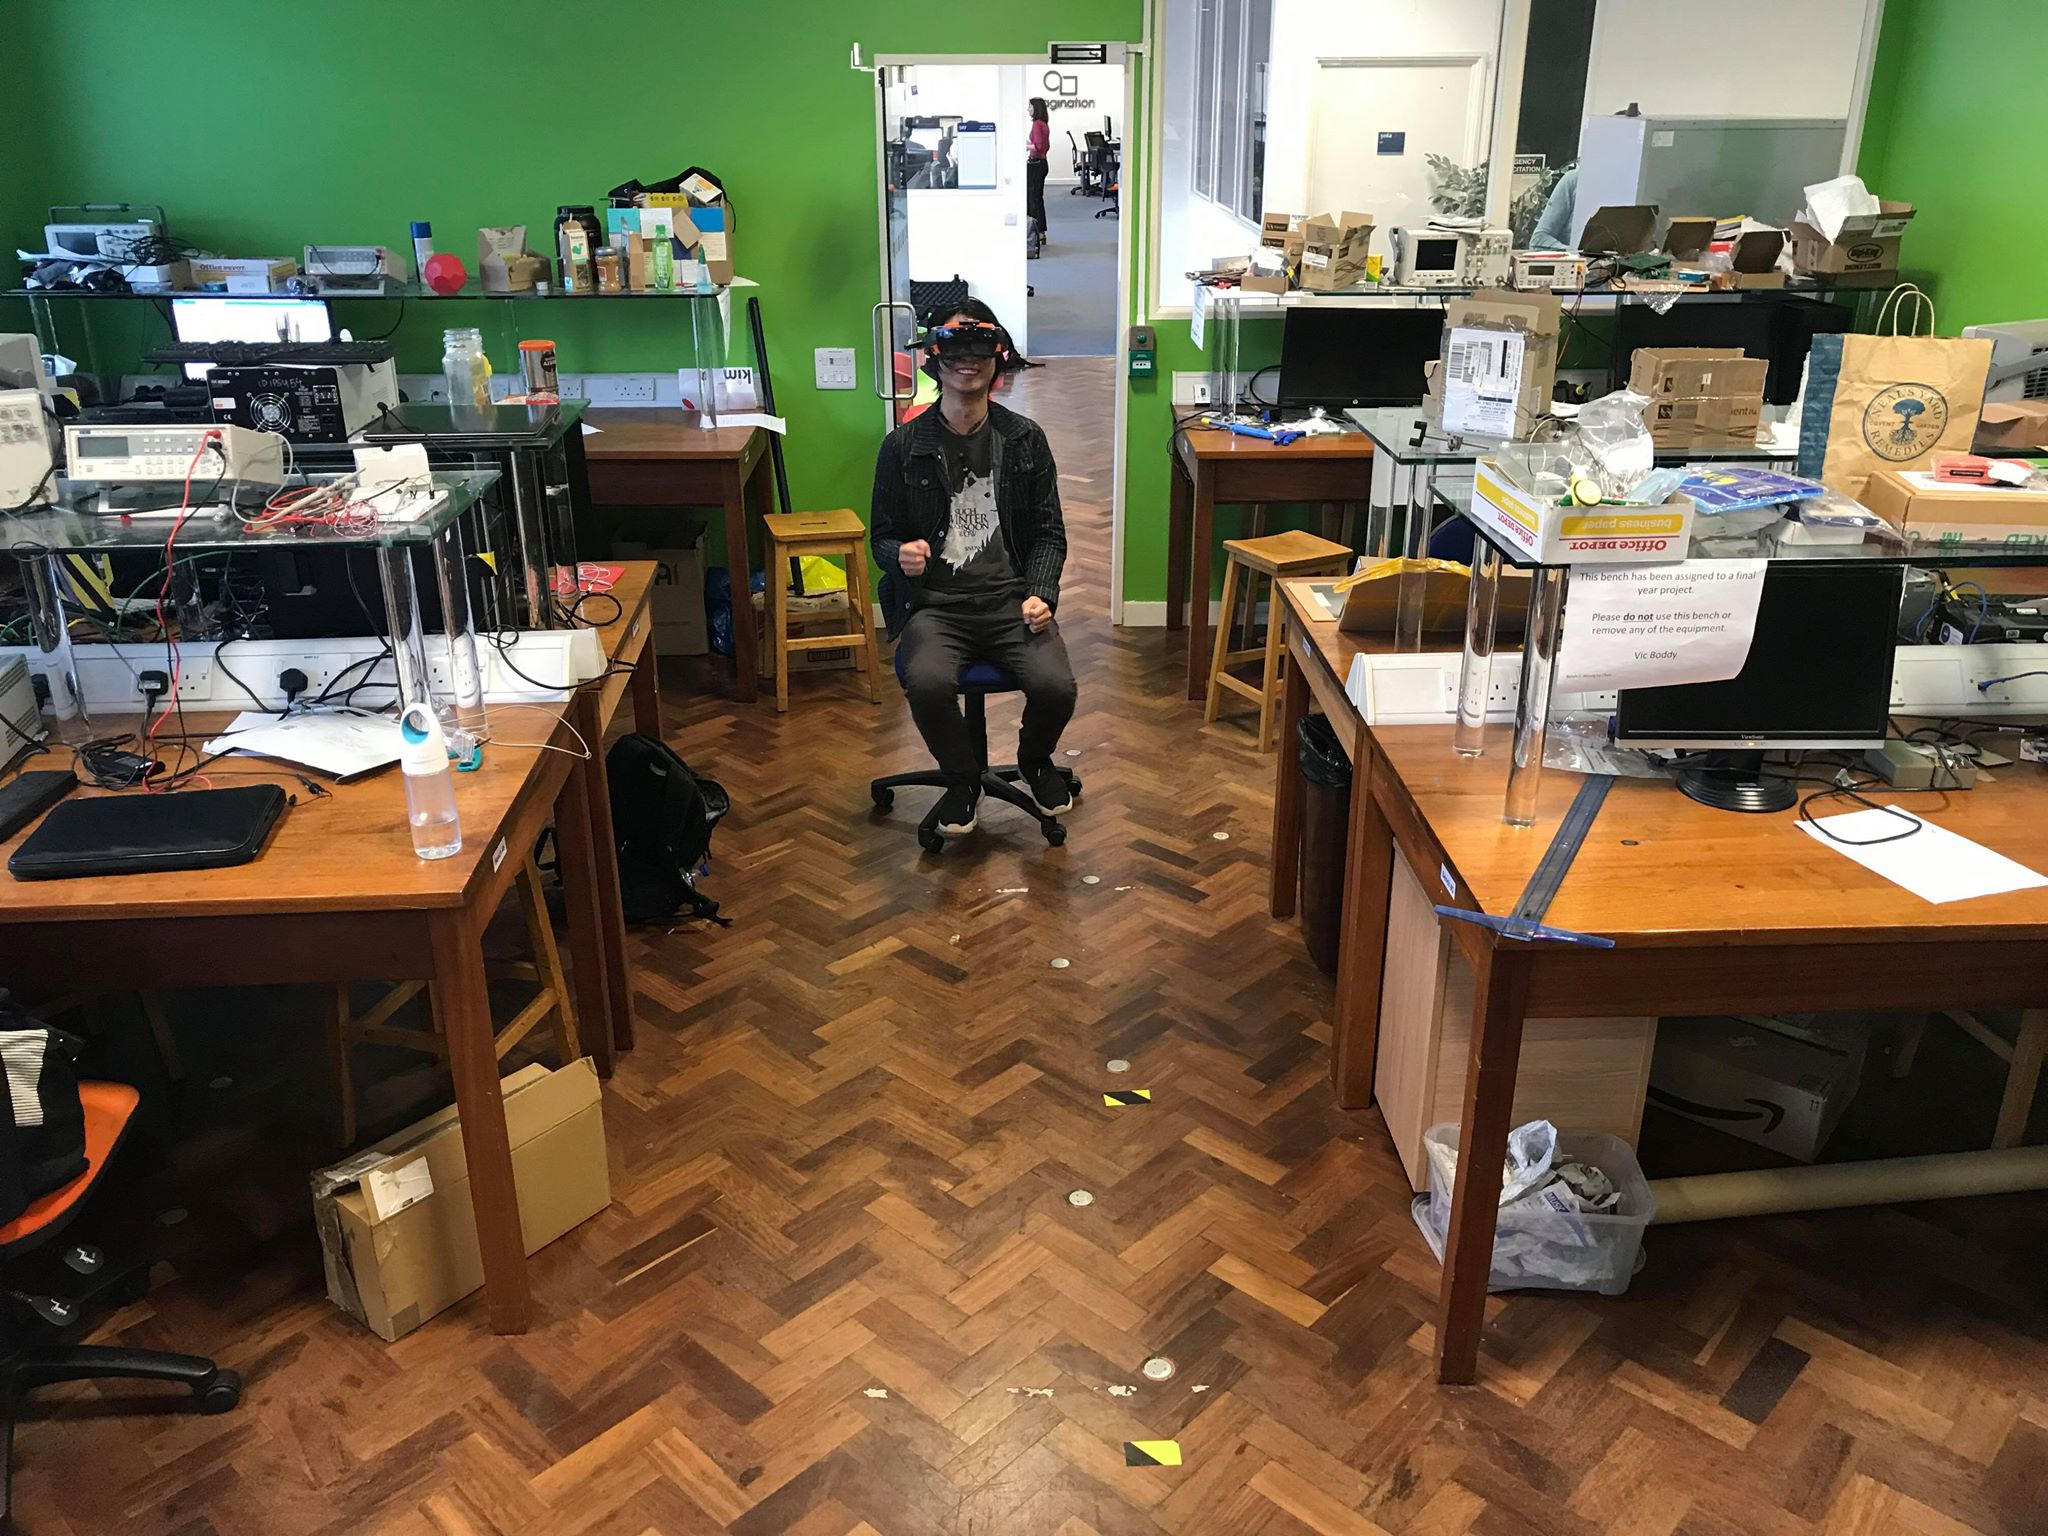
\includegraphics[width=1.0\linewidth,height=41.5mm]{img/chapter6_test/realFront.jpg}
		\caption{Target persons will stand on the markings in front of the test subject which are 1m apart.}
	\end{subfigure}
	\vspace{-1\baselineskip}
	\begin{center}
		\caption{We emulate the real world position of the Gazebo model position in the ICRS lab. We monitor the simulated velocity of the wheelchair as we vary the distance the target person is from the Hololens.}
		\label{fig:greenredrender}
	\end{center}
	\vspace{-2\baselineskip}
\end{figure}

\subsubsection{Real World Lab Setup}
We are trying to test how the velocity of the wheelchair changes when the system detects a collision risk. We model the movement of the wheelchair in the Gazebo simulation, but we need real human detections to test the reactive control system. We use the same setup used in Section \ref{sec:testSetup}, where we use the long hall between benches in the 5th floor ICRS lab to replicate the hallway outside the PRL lab.

\subsubsection{Monitoring ROS Topics}
We record the ROS topics publishing the linear and angular velocities of the simulated wheelchair using a ROS Bag. We monitor the following topics:

\begin{itemize}
	\item \code{/navigation/main\_js\_cmd\_vel}, the velocity controlled by joystick inputs.
	\item \code{/holo/cmd\_vel}, the reactive control velocity.
	\item \code{/arta/cmd\_vel}, the simulated velocity of the wheelchair.
\end{itemize}

\subsection{Test Procedure}
We asked the test subject to sit in a chair in the middle of the hallway wearing the Hololens. Similar to the experiment in Section \ref{sec:testSetup}, the target person stands at different distances to the test subject. Using the keyboard, we control the simulated wheelchair driving it forward down the simulated hallway. At each marked distance, we  record the joystick, reactive control and final velocities of the simulated wheelchair using the ROS bag for comparison. We test distances between $1$ and $4$ meters away, since the reactive control system only takes over for detections closer than $3$ meters. 

\paragraph{}After the distance tests, the test subjects were asked to look to the side as the simulated wheelchair moved forward. We asked the target person to stand to the side of the wheelchair to provide a human detection. This was done to test if the system can realize the detection is not in the trajectory of the wheelchair, and for the system to realize reactive control is not necessary.

\subsection{Results}
We present the results of this experiment in Figure \ref{fig:reactiveResults}. We note at $3$ meters that the reactive control system detects a collision risk and reacts appropriately by reducing the velocity of the wheelchair. We see in Figure \ref{fig:reactiveResults}.a that the output velocity of the reactive control system is below the ideal reactive control velocity of $0.5$m/s. Furthermore, the velocity oscillates between $0.3$m/s and $0.1$m/s, well below the ideal velocity. Figure \ref{fig:reactiveResults}.b shows a similar trend, whereby the output velocity of the reactive control system is $0$m/s instead of the ideal value of approximately $0.1$m/s in the ideal case. Similarly, Figure \ref{fig:reactiveResults}.c also shows a discrepancy. However, more significantly is that there are oscillations in the velocity caused by flickering detections. At a distance of 4 meters, the reactive control was not activated. As such, there is no difference between the joystick input and reactive control velocities, so we omit those results from the figure.

\paragraph{}With respect to the head turning results, we noted that the system was always able to recognize when the test subject was looking forward or to the side, and we noted no change to the joystick inputs when the user was not looking forward. This indicates that the reactive control system is not activated as intended.

\begin{figure}[]
	\begin{subfigure}[b]{1.0\textwidth}
		\centering
		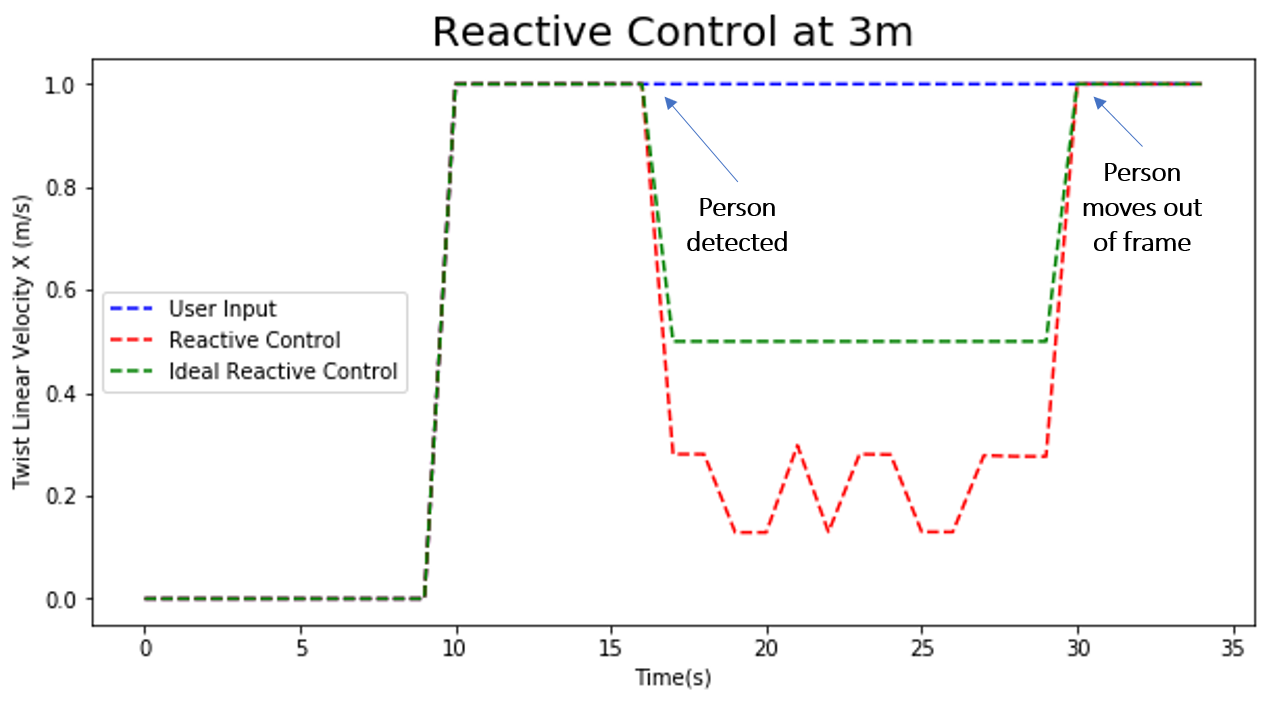
\includegraphics[width=0.75\linewidth]{img/chapter6_test/reactive3.png}
		\caption{Upon detection, the reactive control reduces the velocity to around 0.3m/s. When the collision risk is gone, it returns to 1.0m/s.}
	\end{subfigure}%
	\hspace{\fill} 
	\begin{subfigure}[b]{1.0\textwidth}
		\centering
		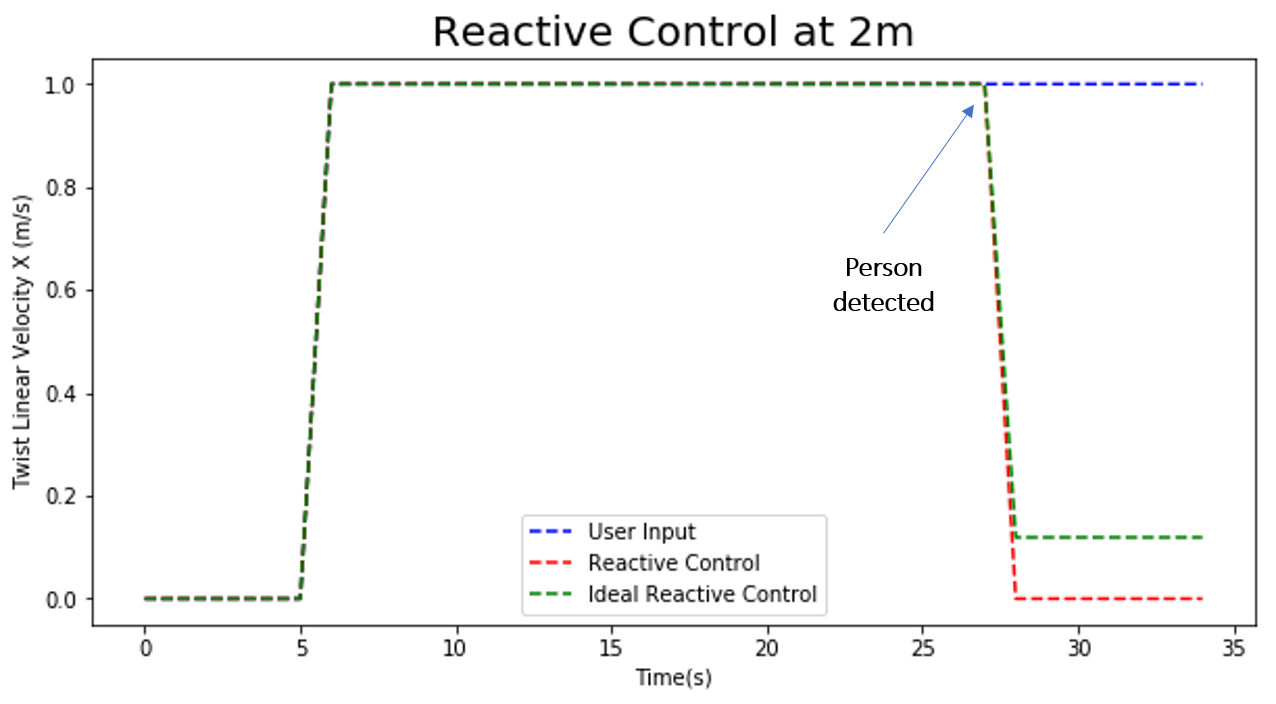
\includegraphics[width=0.75\linewidth]{img/chapter6_test/reactive2.png}
		\caption{At a distance of 2m from the detection, the reactive control system prevents the wheelchair from moving at all.}
	\end{subfigure}
	\begin{subfigure}[b]{1.0\textwidth}
		\centering
		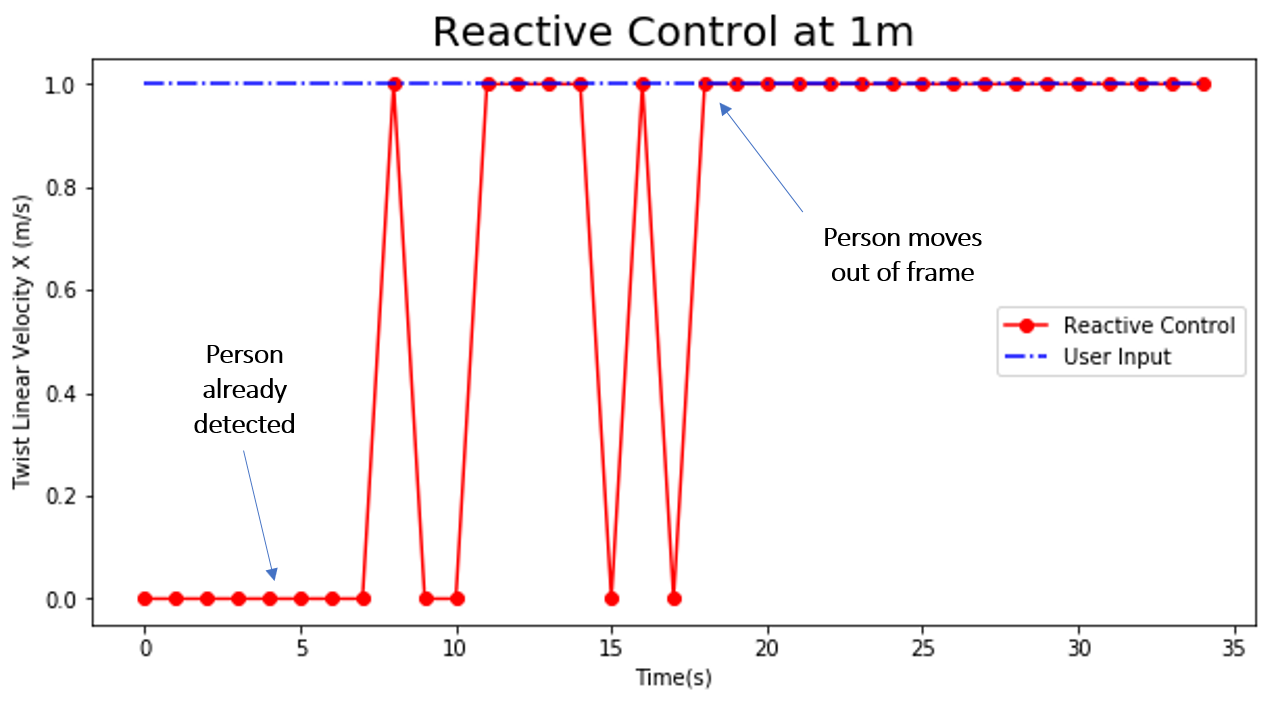
\includegraphics[width=0.75\linewidth]{img/chapter6_test/reactive1.png}
		\caption{The reactive control output velocity oscillates between 0 and 1 due to flickering detections. HDD fails to detect people if they are too close.}
	\end{subfigure}
	\vspace{-1\baselineskip}
	\begin{center}
		\caption{Reactive Control System velocity outputs at different distances.}
		\label{fig:reactiveResults}
	\end{center}
	\vspace{-2\baselineskip}
\end{figure}

\newpage

\subsection{Discussion} \label{sec:gazeboDiscussion}
Due to the issues with hologram placement accuracy discussed in Section \ref{sec:distanceDiscussion}, we can explain the discrepancy between the ideal reactive control velocity and the simulated reactive control. As was discussed in the previous section, the GameObjects and holograms are not always placed in the correct position or on the correct surface. As such, the distance between the PWU and the GameObject in the Unity world varies slightly compared to the real world measurement. When holograms are placed slightly closer to the PWU, the reactive control system responds by reducing the velocity more than the ideal case, as seen in Figure \ref{fig:reactiveResults}.

\paragraph{}We also wish to discuss the oscillations in the velocities set by the reactive control system. For the graph in Figure \ref{fig:reactiveResults}.a, the velocity oscillates within a small range below the ideal reactive control velocity. These small oscillations are most likely caused by flickering holograms. The holograms are ray cast onto the surface of the detected person, however, due to issues with hologram stability at distance, the placement of the hologram and GameObject oscillates between two values. This is rendered to the user as a hologram flickering between two positions on the detected person. As such, the distance between the target and the PWU changes, causing an oscillation in the velocity output of the reactive control system. 

\paragraph{}With regards to the larger oscillations seen in Figure \ref{fig:reactiveResults}.c, we believe that this is caused by the failure of the HDD system to detect a person standing that close to the PWU. However, we are unsure of the root cause of this problem. There is a possibility that this issue is caused by the YOLO detector being unable to detect a person when only their torso and head are visible. The more likely cause is that the OpenPose keypoint estimation fails due to it being unable to estimate the keypoints due to the person being too close. As part of our optimization to run both the tracker and pose estimator on the limited GPU memory, we reduced the network resolution of OpenPose, which results in less accurate key point estimations. The reduction in network resolution may also explain why the HDD system is unable to detect people further away, since the pose estimator fails for persons far away, as seen in Section \ref{sec:keypointEstimate}.

\paragraph{}Finally, we discuss the Hololens and ARTA frame alignment to determine if a detected person is in front of the wheelchair. From the tests, we noticed no change in the forward velocity of the simulated wheelchair. Furthermore, the cursor rendered on the holographic screens changes to the colour red when the PWU is not looking forward, and changes to green when the user is facing forward. This shows that the calibration process and alignment is correct, and that we can now test the full system.

\newpage

\section{Full System}
As a final test, we want to see the whole system in action with all three devices functioning and communicating with each other. We want to check whether the HDD system can detect people who are walking towards the PWU operating ARTA. We also want to see how the reactive control system responds to collision risks in a real world setting, and whether the the response is fast enough to compensate for people walking and the wheelchair moving. This test utilizes ARTA, the HDD system and the Hololens running the full Unity application.

\subsection{Test Setup}
This test was conducted in the hallway outside the Personal Robotics Lab on the 10th floor of the EEE building. The reason for this choice of test location is the pre-existing height maps for localisation and navigation that have been developed by the members of the PRL. Furthermore, this experiment was designed to test the real world application of the Gazebo Simulation test we conducted in Section \ref{sec:gazeboSimTest}.

\paragraph{}This experiment involves positioning ARTA at the end of the hallway. The test subject is sat in the wheelchair wearing the Hololens running the Unity application. Communication between the Hololens and the HDD system is established and checked to ensure the HDD system is receiving video frames and processing them. We then check the Hololens for detections by asking the test subject to confirm they can see holograms being rendered. We then ensure ARTA is communicating with the Hololens by trying to move the wheelchair without any detections and checking the \code{/holo/cmd\_vel/} ROS topic for messages.

\subsection{Test Procedure}
To test the effectiveness of the system, we designed three different scenarios:

\begin{enumerate}
	\item Target Away: ARTA and PWU driving forward in the same direction as the target person walking away down the hallway.
	\item Target Towards: ARTA and PWU driving forward as the target person walks towards the PWU.
	\item Looking Away: ARTA and PWU driving forward, PWU is looking to the side so that the target person is not in the FOV of the Hololens.
\end{enumerate}

We designed these scenarios with the system in mind. We want to test whether the Hololens will detect a person as a collision risk and translate it to a reactive control output that slows down the powered wheelchair, preventing a collision. We illustrate the positions and motions of the target person using the Gazebo simulation map in Figure \ref{fig:fullSystemTest} since it provides an aerial representation of the hallway.

\begin{figure}[ht]
	\centering
	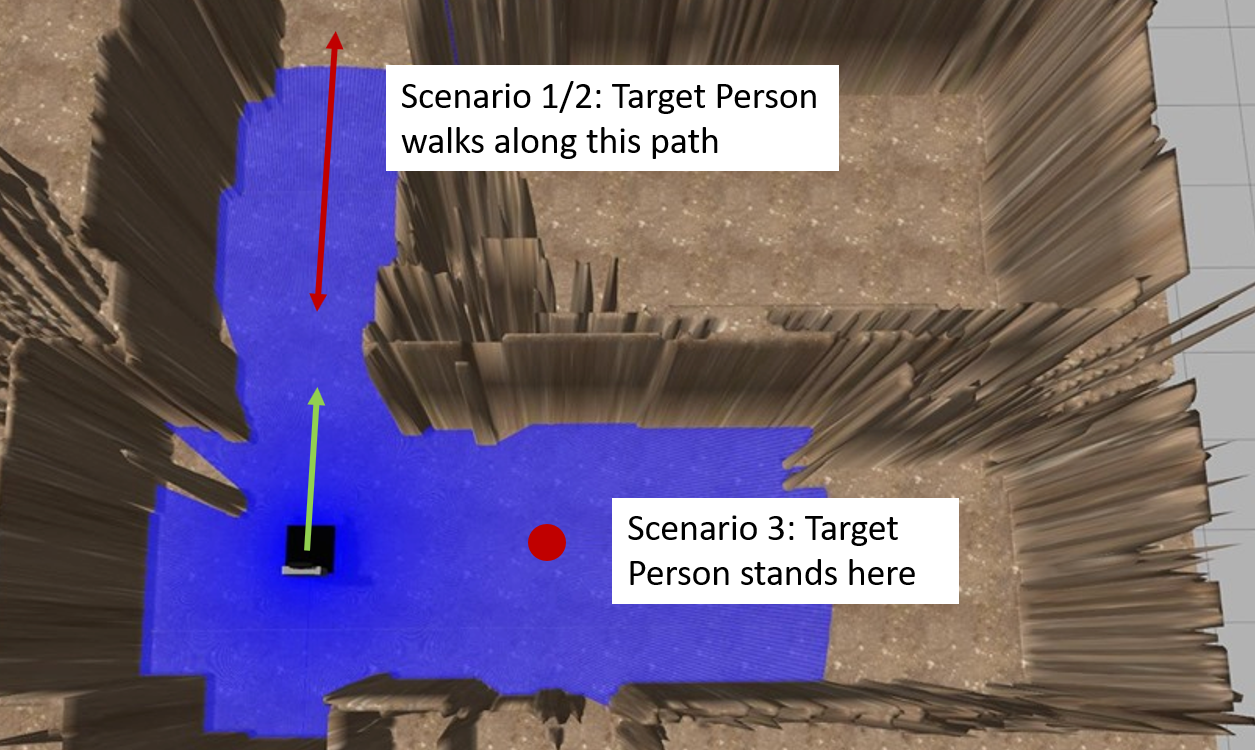
\includegraphics[width=0.9\linewidth]{img/chapter6_test/fullSystem.png}
	\caption{The experimental setup used to test the full system. We ask the target person to walk down the hallway for Scenarios 1 \& 2. For Scenario 3, the target person stands still.}
	\label{fig:fullSystemTest}
\end{figure}

\paragraph{Target Away} In this scenario, we are testing the ability of detecting a person walking in the same direction as the wheelchair. We want to test the system response to the detection which we expect to be a reduction in the forward velocity of ARTA, allowing the robot to continue moving forward, albeit at a slower velocity. We also want to evaluate how the system responds to the person moving out of the frame.

\paragraph{Target Towards} This experiment was designed to test how the system responds to a collision risk that is approaching the wheelchair. The target person is asked to walk towards the wheelchair as the wheelchair moves forward. We are testing for the system to detect the person and rapidly decreasing the forward velocity of the wheelchair as the target person comes closer. We expect the system to stop moving completely when the target person is closer than 2m away.

\paragraph{Looking Away} We ask the test subject wearing the Hololens to drive ARTA in a forward direction while looking to the side. The target person is asked to stand still to the side 2m away from the start position of ARTA and the PWU. This scenario is designed to test how the system is able to recognize the detected person is not in the current trajectory of the wheelchair, and so the reactive control system does not need to modify the user joystick input commands to avoid a collision.

\paragraph{} During Scenarios 1 \& 2, we asked the Target Person to maintain a constant walking speed slightly faster than the top speed of 1.0m/s of the powered wheelchair. We also asked the Target Person to continue walking unless absolutely sure that a collision would occur, in which case we asked the Target Person to avoid the collision themselves.

\begin{figure}[ht]
	\begin{subfigure}[b]{.48\textwidth}
		\centering
		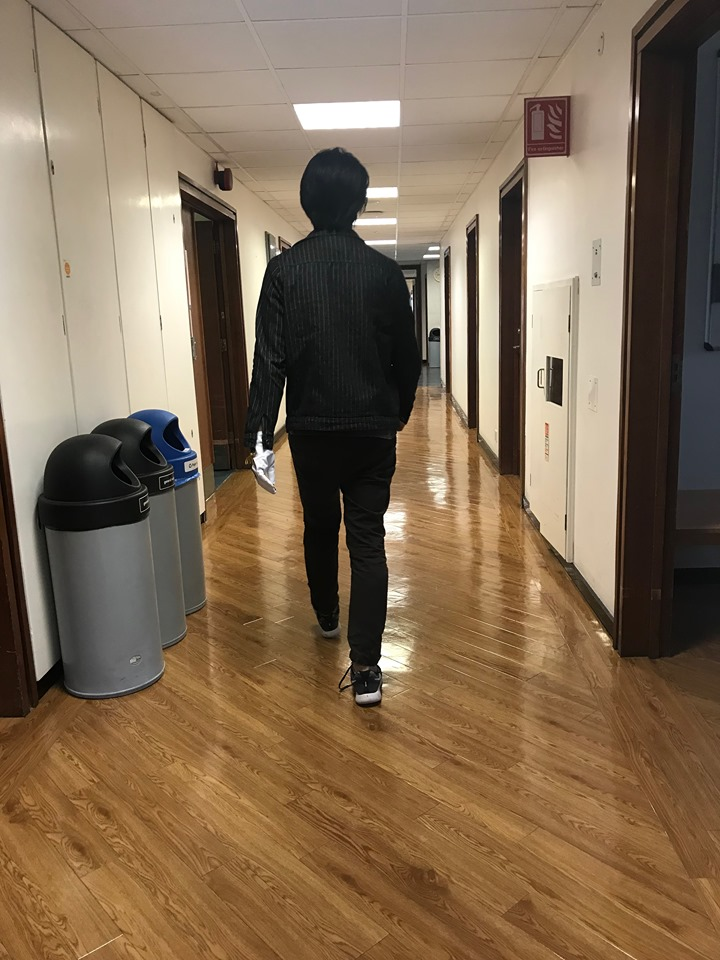
\includegraphics[width=0.5\linewidth]{img/chapter6_test/zihanBack.jpg}
		\caption{Scenario 1: Target person walking in the same direction as forward motion of ARTA.}
	\end{subfigure}%
	\hspace{\fill} 
	\begin{subfigure}[b]{.48\textwidth}
		\centering
		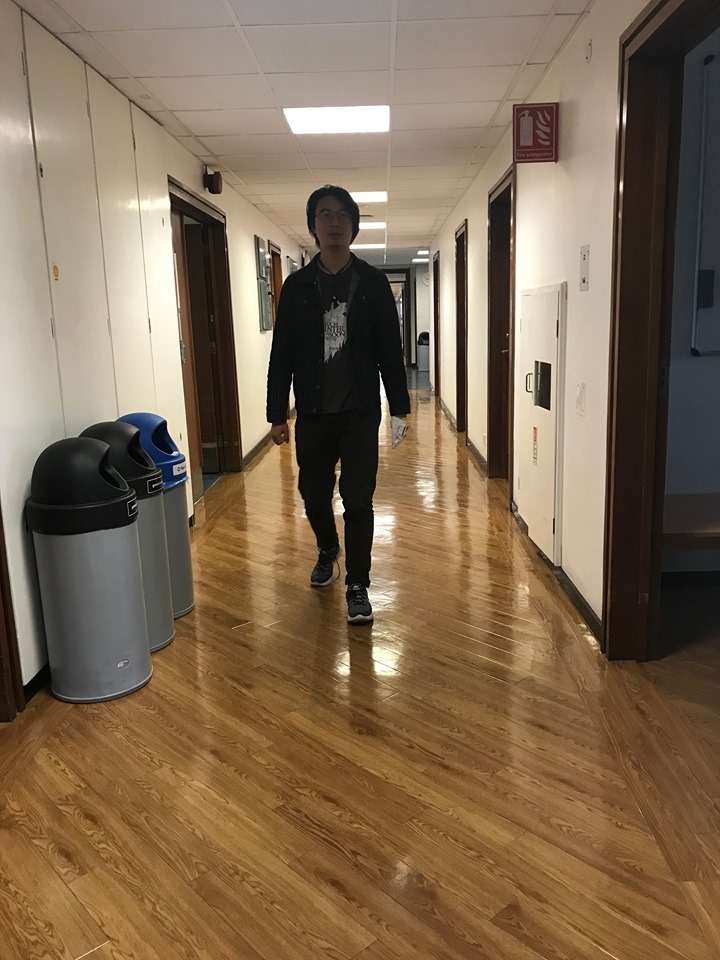
\includegraphics[width=0.5\linewidth]{img/chapter6_test/zihanForward.jpg}
		\caption{Scenario 2: Target person walking towards the PWU and ARTA.}
	\end{subfigure}
	\vspace{-1\baselineskip}
	\begin{center}
		\caption{The path taken by the Target Person along the hallway outside the PRL.}
		\label{fig:zihanBackForward}
	\end{center}
	\vspace{-2\baselineskip}
\end{figure}


\subsection{Results}
We measured the success of a scenario by whether human intervention was required to prevent a collision. We define human intervention as the act of:

\begin{itemize}
	\item The PWU stopping the forward joystick input manually or by navigating the wheelchair out of the way to prevent a collision.
	\item The Target Person having to move themselves off the assigned path to avoid a collision.  
\end{itemize}

\subsubsection{Target Away}
Through our observation of this scenario, we noticed several things:

\begin{itemize}
	\item System was unable to detect target person beyond 3-4 meters in front of the wheelchair.
	\item ARTA moved much slower than expected despite the target being between 2-3m in front of the device.
\end{itemize}

We define a detection as the placement of a hologram at the position of the detected object. The test subject was unable to see a hologram of the green arrow on the surface of the target person when the target person was standing further than 3-4 meters away. The PWU and ARTA retained a relatively smooth velocity behind the target person walking away and no collision with the target occurred. When the target person left the FOV of the PWU, the wheelchair returned to the top velocity of 1m/s.

\subsubsection{Target Towards}
In this scenario, the PWU and ARTA drove forwards as the target person walked towards the powered wheelchair. We noticed that as soon as the target person was approximately 3m away from the PWU, the velocity of ARTA reduced rapidly in a sudden jerking motion. As the target person got closer, we noted that ARTA oscillating between motion and being stationary, instead of remaining completely still. When the target person was very close to the PWU, ARTA began moving forward, indicating the reactive control system had failed to notice a detection and the system required human intervention. 

\subsubsection{Looking Away}
This test involved driving the wheelchair forward while the PWU looked at a target to the side. For this scenario, we noted no change in the velocity as the PWU detected the target person, which indicates that the reactive control system was not activated as expected.

\subsubsection{Summary of Scenarios}
To summarise the results of the scenarios, we want to highlight several points we noticed during the test. Firstly, we want to highlight that the system is able to determine whether a detection is in front of the powered wheelchair and in the way of the current trajectory. However, occasionally the system is unable to detect target persons in front of the wheelchair. This issue was observed when the target was either far away from the PWU or extremely close. Secondly, we note that the reactive control causes a sudden and much more rapid decrease in velocity than we intended. Finally, we want to highlight the issue the system faced when the target person was very close which caused Scenario 2 to require human intervention.

\subsection{Discussion}
We now discuss the issues highlighted in the previous section. We begin with the issue whereby the system fails to detect a target person standing very close to the PWU. As discussed in Section \ref{sec:distanceDiscussion} and Section \ref{sec:gazeboDiscussion}, this is most likely due to a failed detection by the HDD system for people too close to the PWU. This event is similar to the oscillation issue we faced in Section \ref{sec:gazeboDiscussion}, where for close detections, the velocity output of the reactive control system oscillated between 0m/s and 1m/s. 

\paragraph{} Furthermore, due to the variance in hologram placement distance, we can explain the rapid decrease in velocity output at 3m that occurred in Scenario 2. We believe that as the target person crossed the 3m distance and activated the reactive control system, the GameObject representing the person was placed slightly in front of the target. This incorrect placement caused the sudden drop in velocity. In addition, as the distance between the PWU and the target decreased, the ray casting of the GameObject had to correct itself multiple times, causing the distance between them to fluctuate. These fluctuation explain the rapid changes in velocity that caused ARTA to oscillate between movement and remaining stationary.

\paragraph{}As discussed in Section \ref{sec:gazeboDiscussion}, the lack of detections for people far away may be caused by incorrect pose estimations by the OpenPose network in the HDD system due to the low network resolution.

\subsection{Overall System Discussion}
By testing the full system, we were able to assess our implementation in a real world scenario. Although the real world scenario was simplified to only three controlled situations, we immediately noticed that there is a lot of room for improvement. First and foremost is in the HDD system, where persons far away were not recognized. From our tests, we established a possible limiting factor being the resolution of the OpenPose network, which may fail key point estimation for small figures in the distance. Secondly, in the Hololens Unity application, where we convert the image co-ordinate of the detection to a world co-ordinate. Here we rely on the library provided by Vulcan Technologies, which utilizes the camera parameters to form an un-projection matrix to obtain the world position of the pixel. Due to the delay from the streaming to a partner PC and processing through the HDD system, the world co-ordinate is slightly off and not representative of the world position of the person in the current frame. Finally, the rapid decrease in ARTA forward velocity when a detection enters the reactive control activation range. Due to the variance in hologram distance, we realized it was unsuitable to use a scaling function that reduced the speed of the wheelchair so aggressively. We discuss these issues further in the next chapter of the report.
